\documentclass{nicegram}
\usepackage{tikz}
\usepackage{calc}
\usepackage{tikz-3dplot}
\begin{document}
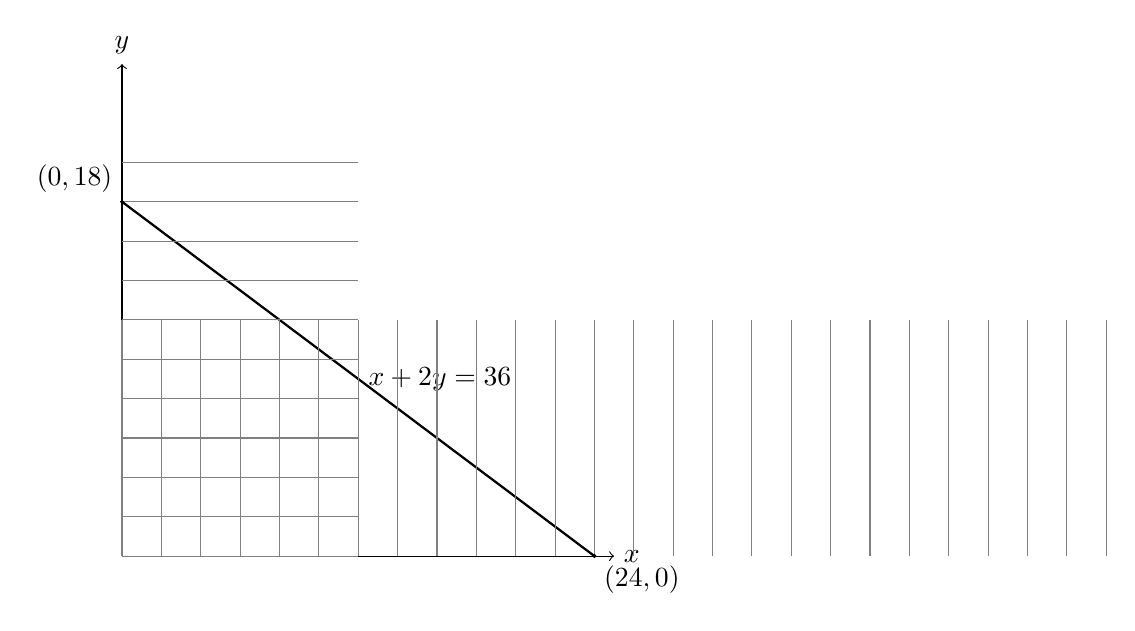
\begin{tikzpicture}[scale=0.25]
    % Draw the axes
    \draw[->] (0,0) -- (0,25) node[above] {$y$};
    \draw[->] (0,0) -- (25,0) node[right] {$x$};

    % Draw the line x + 2y = 36
    \draw[thick] (24,0) -- (0,18) node[midway,right] {$x + 2y = 36$};

    % Draw grid
    \foreach \x in {0,2,...,50} 
        \draw[thin, gray] (\x,0) -- (\x,12);
        
    \foreach \y in {0,2,...,20} 
        \draw[thin, gray] (0,\y) -- (12, \y);

    % Add points on the axes
    \filldraw[black] (24,0) circle (2pt) node[below right] {$(24, 0)$};
    \filldraw[black] (0,18) circle (2pt) node[above left] {$(0, 18)$};
    
\end{tikzpicture}
\end{document}